\section{Einführung}
Ein Stoß zwischen zwei Festkörpern heißt \textbf{gerader} Stoß, wenn beide Geschwindigkeitsvektoren vor dem Stoß parallel zur Stoßgeraden sind. Die Stoßgerade steht dabei senkrecht auf den Oberflächen der beiden Körper am Berührungspunkt. Er heißt \textbf{zentral}, wenn die Schwerpunkte der Körper auf der Stoßgeraden liegen. Wird die kinetische Energie vollständig erhalten, so ist der Stoß \textbf{elastisch}. \\

Da beim Stoß die Summe der äußeren Kräfte auf das Gesamtsystem aus beiden Kugeln 0 ist, bewegt sich der Schwerpunkt geradlinig gleichförmig und die Schwerpunktsgeschwindigkeit $\vec{v}_s$ ist vor und nach dem Stoß dieselbe. Das Schwerpunktssystem kann also als Inertialsystem gewählt werden. Der Energieerhaltungssatz lautet dann:

\begin{equation}
  \frac{1}{2}m_1(\vec{v}_s+\hat{\vec{v}}_1)^2+\frac{1}{2}m_2(\vec{v}_s+\hat{\vec{v}}_2)^2=\frac{1}{2}m_1(\vec{v}_s+\hat{\pvec{v}}'_1)^2+\frac{1}{2}m_2(\vec{v}_s+\hat{\pvec{v}}'_2)^2
  \label{eq:energieerhalt}
\end{equation}
wobei $\hat{\vec{v_1}}, \hat{\vec{v_2}}$ die Geschwindigkeiten der Kugeln im Schwerpunktssystem und  $m_1, m_2$ die Kugelmassen sind. \\

Da auch Impulserhaltung gilt, fallen die gemischten Terme weg:
\begin{gather}
  \frac{1}{2}(m_1+m_2)v_s^2+\frac{1}{2}m_1\hat{v}_1^2+\frac{1}{2}m_2 \hat{v}_2^2+\vec{v}_s(m_1 \hat{\vec{v}}_1+m_2 \hat{\vec{v}}_2)=\\
  \frac{1}{2}(m_1+m_2)v_s^2+\frac{1}{2}m_1\hat{v_1}'^2+\frac{1}{2}m_2 \hat{v}'_2^2+\vec{v}_s(m_1 \hat{\pvec{v}}'_1+m_2 \hat{\pvec{v}}'_2)\\
  \iff \frac{1}{2}(m_1+m_2)v_s^2+\frac{1}{2}m_1\hat{v}_1^2+\frac{1}{2}m_2 \hat{v}_2^2=\frac{1}{2}(m_1+m_2)v_s^2+\frac{1}{2}m_1\hat{v}'_1^2+\frac{1}{2}m_2 \hat{v}'_2^2
\end{gather}
Im Praktikum werden nur gerade, elastische Stöße zwischen zwei Kugeln betrachtet, bei denen die zweite Kugel vor dem Stoß in Ruhe ist: $\vec{v}_2=0$. Sind $\vec{v}_1$ die Geschwindigkeit der ersten Kugel vor dem Stoß, $\pvec{v}'_1$ und $\pvec{v}'_2$ die Kugelgeschwindigkeiten nach dem Stoß, so gilt:

\begin{equation}
  \pvec{v_1}'=\frac{m_1-m_2}{m_1+m_2}\vec{v_1} \qquad \pvec{v_2}'=\frac{2m_1}{m_1+m_2}\vec{v_1}
  \label{eq:stossgeschw}
\end{equation}

Hängen beide Kugeln an einem Pendel der Länge $l$, so berechnet man die resultierende Auslenkung $a_2'$ der gestoßenen Kugel aus der Auslenkung $a_1$ der ersten Kugel vor dem Stoß durch

\begin{equation}
  a_2'=\frac{2m_1}{m_1+m_2}a_1
  \label{eq:auslenkung}
\end{equation}

Rollt die stoßende Kugel vor dem Stoß eine Fallrinne herunter, so ist nur der Translationsanteil der kinetischen Energie für den Stoß relevant. Um den Anteil $\varepsilon$ der Translations- an der kinetischen Energie zu berechnen, benötigt man das Trägheitsmoment einer Kugel (Radius $R$):

\begin{align}
  J_{\text{Kugel}}&=\int_0^{2\pi}\mathrm{d}\varphi\int_0^\pi\mathrm{d}\theta\int_0^R \mathrm{d}r \, r^2 \sin(\theta)r_\bot^2 \rho
  =\int_0^{2\pi}\mathrm{d}\varphi\int_0^\pi\mathrm{d}\theta\int_0^R \mathrm{d}r \, r^4\sin(\theta)^3 \frac{m}{\frac{4}{3}\pi R^3} \\
  &=\frac{1}{5}R^5 \cdot 2\pi\cdot \frac{4}{3}\cdot \frac{m}{\frac{4}{3}\pi R^3} = \frac{2}{5}mR^2
  \label{eq:traegheitsmom}
\end{align}
Dabei wurde genutzt, dass 
\begin{equation}
  \int_0^\pi \, \mathrm{d}\theta\, \sin(\theta)^3=\int_0^\pi \, \mathrm{d}\theta\, \sin(\theta) - \int_0^\pi \, \mathrm{d}\theta\, \cos(\theta)^2 \sin(\theta)\overset{u = \cos(\theta)}{=}2-\int_{-1}^1 \, \mathrm{d}u \, u^2 =2 - \frac{2}{3}=\frac{4}{3}
  \label{eq:sinintegral}
\end{equation}

So ist die resultierende Auslenkung der Kugel am Pendel:
\begin{equation}
  a_2'=\frac{2m_1}{m_1+m_2}\sqrt{\varepsilon 2lh}
  \label{eq:fallrinne}
\end{equation}

mit $\varepsilon=5/9$.\\

Ziel der Versuche ist nun, die aus den Stoßgesetzen hergeleiteten Beziehungen experimentell zu überprüfen.

\section{Versuch: Gerader zentraler Stoß beim ballistischen Pendel}

Die große (Masse $m_g=\SI{486.42\pm0.01}{g}$) und die mittlere Kugel (Masse $m_m=\SI{175.59\pm0.01}{g}$) hängen jeweils an einem an der Decke befestigtem Fadenpendel der Länge $l=\SI{1.922\pm0.01}{m}$. Sie sind so justiert, dass die Kugel sich in der Ruheposition gerade mittig berühren und die Stoßgerade in der Pendelebene liegt. Unter den Kugeln ist parallel zur Stoßgeraden ein Längenmaß angebracht. Durch zwei Schieber auf der Messlatte werden Auslenkungen gemessen und der Versuch wird für 5 verschiedene Auslenkungen je 5 mal durchgeführt.\\

Es wird erwartet, dass aufgrund der Impulserhaltung die schwerere Kugel eine stärkere Auslenkung der leichteren hervorruft als andersherum. Aus gleichem Grund wird bei größerer Auslenkung der stoßenden Kugel eine größere Auslenkung der gestoßenen Kugel erwartet.

Zunächst ist die mittlere Kugel in Ruhe und die große Kugel wird zum Stoß ausgelenkt (Fehler jeweils \SI{\pm0.1}{cm}):

\begin{table}[H]
  \centering
  \begin{tabular}{c | c | c | c | c | c | c}
    \diagbox{\small{Ausl.}}{Stoß} & 1 & 2 & 3 & 4 & 5 & Mittelwert \\ \hline
    \SI{1}{cm} & \SI{1.3}{cm} & \SI{1.5}{cm} & \SI{1.4}{cm} & \SI{1.6}{cm} & \SI{1.5}{cm} & \SI{1.5\pm0.2}{cm} \\
    \SI{2}{cm} & \SI{3.0}{cm} & \SI{3.1}{cm} & \SI{3.0}{cm} & \SI{2.9}{cm} & \SI{2.9}{cm} & \SI{3.0\pm0.1}{cm} \\
    \SI{5}{cm} & \SI{7.0}{cm} & \SI{7.4}{cm} & \SI{7.3}{cm} & \SI{7.3}{cm} & \SI{7.3}{cm} & \SI{7.3\pm0.2}{cm} \\
    \SI{10}{cm} & \SI{14.3}{cm} & \SI{14.5}{cm} & \SI{14.4}{cm} & \SI{14.5}{cm} & \SI{14.4}{cm} & \SI{14.4\pm0.1}{cm} \\
    \SI{15}{cm} & \SI{21.5}{cm} & \SI{21.5}{cm} & \SI{21.4}{cm} & \SI{21.6}{cm} & \SI{21.4}{cm} & \SI{21.5\pm0.1}{cm}
  \end{tabular}
  \caption{Große stößt mittlere}
  \label{tab:grossgegenmittel}
\end{table}
Jetzt mit vertauschten Rollen:
\begin{table}[H]
  \centering
  \begin{tabular}{c | c | c | c | c | c | c}
    \diagbox{\small{Ausl.}}{Stoß} & 1 & 2 & 3 & 4 & 5 & Mittelwert \\ \hline
    \SI{1}{cm} & \SI{.5}{cm} & \SI{.6}{cm} & \SI{.6}{cm} & \SI{.5}{cm} & \SI{.7}{cm} & \SI{.6\pm.1}{cm} \\
    \SI{2}{cm} & \SI{1.3}{cm} & \SI{1.3}{cm} & \SI{1.2}{cm} & \SI{1.0}{cm} & \SI{1.0}{cm} & \SI{1.2\pm.2}{cm} \\
    \SI{5}{cm} & \SI{2.8}{cm} & \SI{2.7}{cm} & \SI{2.8}{cm} & \SI{2.6}{cm} & \SI{2.6}{cm} & \SI{2.7\pm.2}{cm} \\
    \SI{10}{cm} & \SI{5.6}{cm} & \SI{5.4}{cm} & \SI{5.3}{cm} & \SI{5.3}{cm} & \SI{5.3}{cm} & \SI{5.4\pm.2}{cm} \\
    \SI{15}{cm} & \SI{8.0}{cm} & \SI{8.3}{cm} & \SI{7.9}{cm} & \SI{8.1}{cm} & \SI{7.9}{cm} & \SI{8.0\pm.2}{cm}
  \end{tabular}
  \caption{Mittlere stößt große}
  \label{tab:mittelgegengross}
\end{table}
Aus \cref{eq:auslenkung} wird ein linearer Zusammenhang zwischen den Auslenkungen der stoßenden und der gestoßenen Kugel erwartet. Die Steigung für die Daten aus dem ersten Durchlauf sollte größer sein, denn die Masse $m_1$ der stoßenden Kugel trägt als Faktor in \cref{eq:auslenkung} zur Steigung bei.
\begin{figure}[H]
  \centering
  \begin{tikzpicture}
    \begin{axis}[
      width=15 cm,
      height=10 cm,
      xmin=1, xmax=15,
      ymin=0, ymax=25,
      xlabel={Auslenkung stoßende Kugel [cm]},
      ylabel={Auslenkung gestoßene Kugel [cm]},
      legend entries={Große $\rightarrow$ mittlere, Mittlere $\rightarrow$ große}
    ]
      \addplot[mark=x, only marks, error bars/.cd, x dir=both, x fixed=0.1, y dir=both, y explicit] table[y error index=2] {grossgegenmittel.txt};
      \addplot[mark=o, only marks, error bars/.cd, x dir=both, x fixed=0.1, y dir=both, y explicit] table[y error index=2] {mittelgegengross.txt};
    \end{axis}
  \end{tikzpicture}
  \caption{Stoßversuch am Pendel}
  \label{fig:pendelstoss}
\end{figure}

Mit \emph{gnuplot} werden nach dem \emph{least-squares}-Verfahren die Werte gegen die Funktion $f(x)=k\cdot x$ gefittet. Ausgabe:

\begin{table}[H]
  \centering
  \begin{tabular}{l | c | c}
    Versuch & Wert für $k$ & Varianz der Residuen \\ \hline
    Große $\rightarrow$ mittlere & $k_1=\num{1.44\pm0.02}$ & \num{0.60} \\
    Mittlere $\rightarrow$ große & $k_2=\num{.54\pm0.02}$ & \num{.22}
  \end{tabular}
  \caption{Linearer Fit der Auslenkung}
  \label{tab:pendelstossfit}
\end{table}
Stellt man \cref{eq:auslenkung} um, so sieht man 
\begin{itemize}
  \item Die Summe der Steigungen sollte 2 ergeben:
    \begin{align}
      k_1&=\frac{2m_g}{m_m+m_g} \qquad k_2=\frac{2m_m}{m_m+m_g} \\
      k_1&+k_2=\frac{2m_m+2m_g}{m_m+m_g}=2
      \label{eq:steigungssumme}
    \end{align}
  \item Das Massenverhältnis entspricht dem Verhältnis der Steigungen:
    \begin{equation}
      \frac{k_1}{k_2}=\frac{2m_g}{m_m+m_g}\frac{m_m+m_g}{2m_m}=\frac{m_g}{m_m}
      \label{eq:massenverhaeltnis}
    \end{equation}
\end{itemize}
Jetzt mit Messwerten:
\begin{align}
  k_1+k_2&=\num{1.45\pm0.02}+\num{0.44\pm0.02}=\num{1.98\pm0.03} \\
  \frac{m_g}{m_m}&=\frac{\SI{486.42\pm.01}{g}}{\SI{175.59\pm.01}{g}}=\num{2.7702\pm0.0002} \\
  \frac{k_1}{k_2}&=\frac{\num{1.44\pm0.02}}{\num{0.54\pm0.02}}=\num{2.67\pm0.11}
  \label{eq:steigungsauswertung}
\end{align}
Im Rahmen des Fehlers ist die Summe der Steigungen wie erwartet 2. Das Massenverhältnis aus den gewogenen Massen stimmt innerhalb des Fehlers mit dem Verhältnis der Steigungen überein.\\

\section{Versuch: Gerader zentraler Stoß einer rollenden Kugel}
Bei diesem Versuch wird die kleine Kugel($m_{\text{klein}}= 63,26 \pm 0,01 g $ und $D_{\text{klein}}=2,4 \pm 0,1 cm$) eine Rampe herunter gerollt und regt in einem geraden zentralen Stoß die große, an einem Pendel ($l=1,922 \pm 0,01m$) hängende Kugel ($m_{\text{groß}}=486,42 \pm 0,01g$ und $D_{\text{groß}}=4,7 \pm 0,1 cm$) an.

\begin{figure}[htbp] 
  \centering
	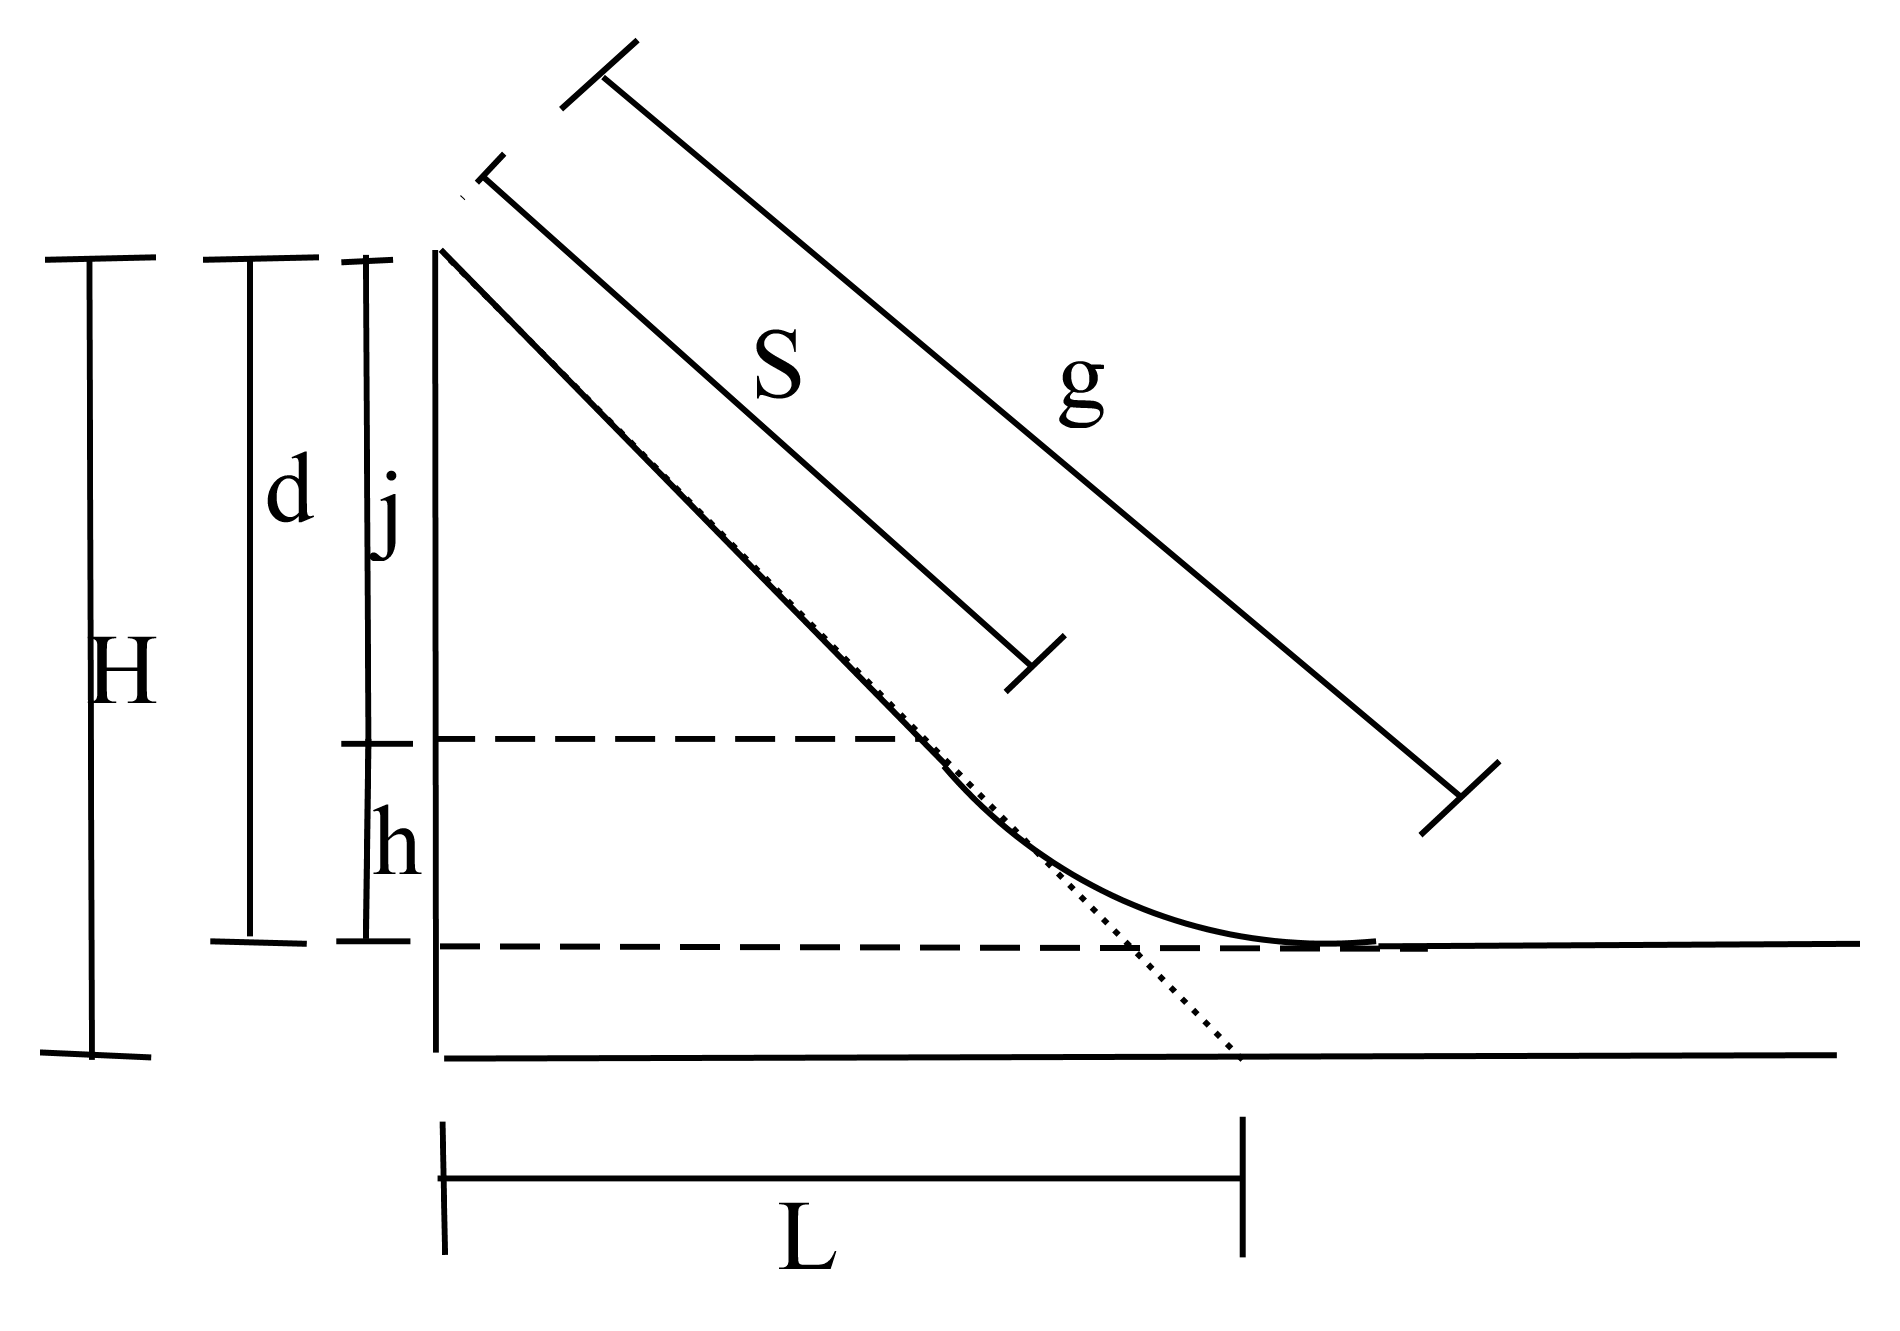
\includegraphics[width=0.7\textwidth]{Fallrinne.png}
	\caption{Schematische Darstellung der Fallrinne}
  \label{fig:Fallrinne}
\end{figure}

Aus Formatierungsgründen wurde in Abbildung \ref{fig:Fallrinne} anstatt $h_0$ (vgl. Versuchsanleitung) $d$ verwendet.

Dieser Versuch wird mit unterschiedlichen Werten für S wiederholt und die entsprechenden maximalen Auslenkungen der großen Kugel werden jeweils durch peilen auf ein auf der Arbeitsfläche liegendes Lineal bestimmt.

\begin{table}[H]
  \centering
  \begin{tabular}{l | c | c | c | c | c | c}
    S [$\pm 0,1$ cm]  & \num{0} & \num{10} & \num{20} & \num{30} & \num{40} & \num{50}\\ \hline
   Durchschnittliche Auslenkung [$\pm 0,2$ cm] & \num{15,26} & \num{14,26} & \num{12,38} & \num{10,64} & \num{8,2} & \num{5,16} \\
   Mittlere Abweichung [cm] & \num{0,128} &\num{0,088} & \num{0,104} & \num{0,112} & \num{0,08} & \num{0,048}
    
  \end{tabular}
  \caption{Auslenkung der grossen Kugel}
  \label{tab:auslenkgross}
\end{table}

Die Fallhöhe $h$ der kleinen Kugel ergibt sich aus $H=32,5 \pm0,2 cn$, $h_0=31,4 \pm 0,3cm$ und $L= 47,8 \pm 0,3cm$ nach der Formel
\begin{equation}
\label{eq:h}
h=h_0-\frac{S}{\sqrt{1+\frac{L^2}{H^2}}}
\end{equation}
in Abhängigkeit von $S$.

Diese Formel erhält man durch Nutzen des Strahlensatzes
\begin{equation}
\frac{S}{g}=\frac{j}{H} \iff j=\frac{S\cdot H}{g},
\label{eq:Strahl}
\end{equation}
des Satzes des Pythagoras
\begin{equation}
g^2=H^2+L^2 \iff g=\sqrt{H^2+L^2}
\label{eq:pytha}
\end{equation}
und der allgemeinen Beziehung
\begin{equation}
h=h_0-j.
\label{eq:einfach}
\end{equation}
Wenn man nun \ref{eq:pytha} in \ref{eq:Strahl} einsetzt und dies in \ref{eq:einfach}, erhält man \ref{eq:h}.
\\

Durch Einsetzen der Werte in \ref{eq:h} erhält man für h
\begin{table}[H]
  \centering
  \begin{tabular}{l | c | c | c | c | c | c}
    S [$\pm 0,1$ cm]  & \num{0} & \num{10} & \num{20} & \num{30} & \num{40} & \num{50}\\ \hline
    h [cm] & \num{31,4} & \num{25,77} & \num{20,15} & \num{14,53} & \num{8,91} & \num{3,29} \\
    
  \end{tabular}
  \caption{h in Abhängigkeit von S}
  \label{tab:hvons}
\end{table}
Der Fehler der Fallhöhe $\Delta h$ ist gleich
\begin{gather}\label{eq:Fehler}
\Delta h= \sqrt{(\frac{\partial h}{\partial h_0}\cdot\Delta h_0)^2+(\frac{\partial h}{\partial S}\cdot\Delta S)^2+(\frac{\partial h}{\partial L}\cdot\Delta L)^2+(\frac{\partial h}{\partial H}\cdot\Delta H)^2}\\
\frac{\partial h}{\partial h_0}\cdot\Delta h_0= \Delta h_0 \\
\frac{\partial h}{\partial S}\cdot\Delta S =-\frac{\Delta S}{\sqrt{1+\frac{L^2}{H^2}}}\\
\frac{\partial h}{\partial L}\cdot\Delta L = \frac{LS\Delta L}{H^2\sqrt{1+\frac{L^2}{H^2}}^3}\\
\label{eq:Fehler2}\frac{\partial h}{\partial H}\cdot\Delta H = \frac{L^2S\Delta H}{H^3\sqrt{1+\frac{L^2}{H^2}}^3}
\end{gather}

Durch Einsetzen der Werte in \ref{eq:Fehler} bis \ref{eq:Fehler2} erhält man für
\begin{table}[H]
  \centering
  \begin{tabular}{l | c | c | c | c | c | c}
    S [$\pm 0,1$ cm]  & \num{0} & \num{10} & \num{20} & \num{30} & \num{40} & \num{50}\\ \hline
  $\Delta h $ [cm] & \num{0,31} & \num{0,31} & \num{0,31} & \num{0,32} & \num{0,33} & \num{0,34} \\
    
  \end{tabular}
  \caption{Fehler in h in Abhängigkeit von S}
  \label{tab:fehlerh}
\end{table}

\begin{figure}[H]
  \centering
  \begin{tikzpicture}
    \begin{axis}[
      width=15 cm,
      height=10 cm,
      xmin=0, xmax=6,
      ymin=0, ymax=18,
      xlabel={Wurzel der Fallhöhe [Wurzel(cm)]},
      ylabel={Auslenkung der Großen Kugel [cm]}
    ]
     \addplot[mark=x, only marks, error bars/.cd, y dir=both, y fixed=0.2, x dir=both, x fixed=0.32] table {wurzelh.txt};
    \end{axis}
  \end{tikzpicture}
  \caption{Auslenkung der großen Kugel gegen die Wurzel der Fallhöhe}
  \label{fig:auslenkung}
\end{figure}

Mit \emph{gnuplot} werden nach dem \emph{least-squares}-Verfahren die Werte gegen die Funktion $f(x)=k\cdot x$ gefittet. Ausgabe:

\begin{table}[H]
  \centering
  \begin{tabular}{l | c | c}
    Variabel & Wert & Varianz der Residuen \\ \hline
    k & \num{2.7673} $\pm0.01601$  & \num{0.0266716} 
  \end{tabular}
  \caption{Linearer Fit der Auslenkung}
  \label{tab:durchbiegungsfit}
\end{table}

Mit der Formel \ref{eq:fallrinne} kann man nun den nutzbaren Energiefaktor $\epsilon$ bestimmen.
\begin{gather}
a'_2=\frac{2m_1}{m_1+m_2}\sqrt{\epsilon 2lh}
\end{gather}\begin{gather*}
\iff \frac{a'_2}{\sqrt{h}}=k=\frac{2m_1}{m_1+m_2}\sqrt{\epsilon 2l}\\
\iff \epsilon = k \frac{2m_1}{m_1+m_2}\sqrt{\frac{1}{2l}}= 0,6132
\end{gather*}

Bei dem Vergleich mit dem Literaturwert $\epsilon_{lit}=\frac{5}{9}$, erhält man
\begin{gather}
\frac{\epsilon}\epsilon_{lit}=1,103\\
\epsilon - \epsilon_{lit}= 0,058
\end{gather}
\section{Abschließende Diskussion}
\subsection{Stoß zweier Kugeln am Pendel}
Dieser Versuch zeigt, dass die aus den Stoßgesetzen hergeleitete Auslenkungsgleichung~\cref{eq:auslenkung} korrekt ist. Es besteht ein linearer Zusammenhang zwischen Auslenkung der stoßenden und der gestoßenen Kugel. Der Proportionalitätsfaktor $k=\frac{2m_1}{m_1+m_2}$ hängt wie erwartet direkt mit den Massen der Kugeln zusammen und das Massenverhältnis lässt sich aus dem Steigungsfit zurückgewinnen.
Der relative Fehler des gewogenen Massenverhältnisses zur Steigung beträgt
\begin{equation}
  \Delta k = \frac{m_g/m_m-k_1/k_2}{m_g/m_g}=\SI{3.62}{\percent}
  \label{eq:steigungsfehler_rel}
\end{equation}
Dieser geringe Fehler ist erstaunlich, da dieselbe Messmethode zum Ablesen der Auslenkung verwendet wurde wie in Versuch 2, wo eine deutlich höhere Differenz zum Theoriewert besteht (s.u.). Möglicherweise ist dies auf einen Wechsel der messenden Person zurückzuführen (Versuch 1: Josh misst, Alex stößt; Versuch 2: Alex misst, Josh lässt Kugel rollen).
\subsection{Gerader zentraler Stoß einer rollenden Kugel}
Bei dem Versuch ,,Gerader zentraler Stoß einer rollender Kugel'' ist eine deutliche Abweichung zum Literaturwert festzustellen, mehr als $10\%$. Dies ist auf die vielen Messwerte mit ihren teilweise nicht kleinen Messungenauigkeiten, die in die Bestimmung von k und damit $\epsilon$ einlaufen, zurückzuführen. Dazu gehört zum Beispiel die Fallhöhe h mit einem Fehler von mehr als $1\%$ und die Auslenkung der großen Kugel mit einem Fehler von $1,3\%$.
Die Bestimmung dieser Auslenkung war in diesem Versuch leider nicht ideal gelöst, da nur zwei Möglichkeiten, die jedoch beide Nachteile hatten, bestanden, sie zu bestimmen.
\begin{enumerate}
\item Auslenkung anpeilen\\
Bei dieser Methode wird die maximale Auslenkung dadurch bestimmt, dass parallel zur Schwingungsrichtung ein Schieber soweit verschoben wird, dass er sich auf einer Höhe mit der Kugel in ihrem Maximum befindet. Der deutliche Nachteil dieser Methode ist das Peilen, da es schwer ist genau das Maximum als Referenzpunkt zu finden und diesen Abstand dann noch genau zu bestimmen.
\item Auslenkung ablesen\\
Bei dieser Methode wurde ein Schieber in den Schwingungsweg der Kugel gestellt und so verschoben das die Kugel diesen möglichst gerade nicht mehr trifft. Dies verdeutlicht auch direkt die Schwäche dieser Methode, es ist sehr schwer den genauen Punkt zu finden, bei dem die Kugel den Schieber so gerade nicht mehr erreicht. Dafür war jedoch das Ablesen der bestimmten Auslenkung deutlich genauer.
\end{enumerate}
Da beide Methoden einen Fehler, der schwer abzuschätzen ist, haben und so für eine große Messungenauigkeit sorgen, sind sie beide nicht besonders gut geeignet. Jedoch standen andere Methoden nicht zur Option.

\nocite{anleitung-ws2014}
